\documentclass[12pt]{article}

% The preceding line is only needed to identify funding in the first footnote. If that is unneeded, please comment it out.
\usepackage{cite}
\usepackage{amsmath,amssymb,amsfonts}
\usepackage{algorithm}
\usepackage{algorithmic}
\usepackage{graphicx}
\usepackage{textcomp}
\usepackage{xcolor}
\usepackage{colortbl}
\usepackage{float}
\usepackage{subcaption}
\usepackage{multirow}

\def\BibTeX{{\rm B\kern-.05em{\sc i\kern-.025em b}\kern-.08em
    T\kern-.1667em\lower.7ex\hbox{E}\kern-.125emX}}
\begin{document}

\title{Coursework of Machine learning cousework 2}



\author{Chen Ting Hung} {}
	
\maketitle

\begin{abstract}
This is the report of out machine learning cousework
\end{abstract}

\section{Subtask 1}
Implement ICM for a binary image that you have corrupted with noise, show the result for a set of images with different noise levels. How many passes through the nodes do you need until you are starting to get descent results?\\

a) a set of images\\
\begin{figure}[htb]
\centering
\begin{subfigure}[b]{.48\linewidth}
  \centering
  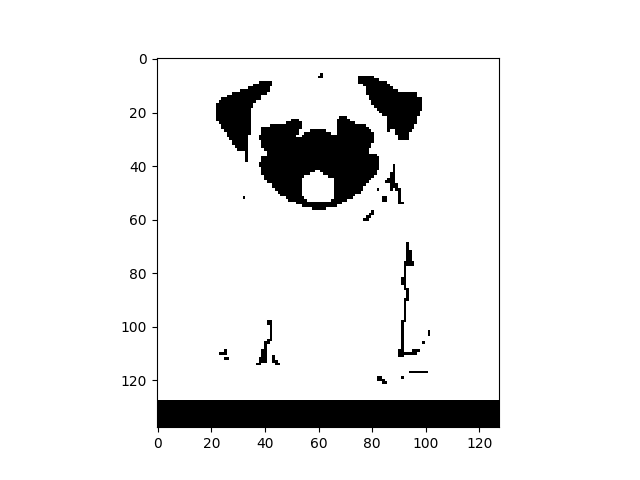
\includegraphics[width=\linewidth]{result/restore0-1.png}
  \caption{\textbf{\texttt{restore0-1.jpg}}}
\end{subfigure}
\label{fig:1}
\end{figure}

b) How many passes through the nodes\\
we do the three different level of gaussian noises all of propotion are setted as 0.7.\\ 
First time is use 0.1 as varSigma, second time is 0.3 and third time is 0.5.\\
We notice that with the noise larger it might increse amount of nodes.\\
Finally, we notice that most of the progress will end around passed through 10 nodes.\\

\section{Subtask 9}

\end{document}
